\documentclass[12pt,letterpaper]{report}
\usepackage[utf8]{inputenc}
\usepackage[spanish]{babel}
\usepackage{amsmath}
\usepackage{amsfonts}
\usepackage{amssymb}
\usepackage{graphicx}
\usepackage[left=2cm,right=2cm,top=2cm,bottom=2cm]{geometry}
\author{Jose Antonio Olvera Gonzalez }
\title{Aplicacniones de los manipuladores parelelos }
\begin{document}
\begin{center}
\textbf{Aplicación de los Robots Paralelos }
\end{center}
APLICACIONES INICIALES 
\begin{flushleft}
Un robot paralelo consiste de una plataforma móvil unida a una plataforma fija mediante una serie de cadenas cinemáticas llamadas piernas. Partiendo del anterior concepto, Bonev establece que el origen del robot paralelo se encuentra en la industria del entretenimiento, siendo James E. Gwinnett en el año 1928 uno de los pioneros en patentar un artefacto basado en el concepto de robot paralelo. La Figura 1 presenta un esquema incluido en el documento de la patente original.\\
La primera aplicación industrial conocida del robot paralelo, siguiendo la cronología propuesta por Bonev, fue  presentada por Willard L.V. Pollard en el año 1940. El dispositivo fue propuesto para pintar vehículos de forma automática con  pintura de aerosol y posteriormente fue patentado como dispositivo para controlar el posicionamiento de una herramienta. El diseño presenta tres motores que determinan la posición de la cabeza de la herramienta, y otros dos motores que mediante un sistema de cables transmite el movimiento que permite orientar la herramienta. \\
Más tarde en la década de los 50, Eric Gough un ingeniero automotriz trabajando en la fábrica de neumáticos de la Ford Dunlop en Birmingham, Inglaterra, desarrolla una máquina Universal de pruebas de neumáticos. . La plataforma fue puesta en funcionamiento en el año 1954 y cumplía la función de probar mecánicamente neumáticos mediante la aplicación de cargas. 
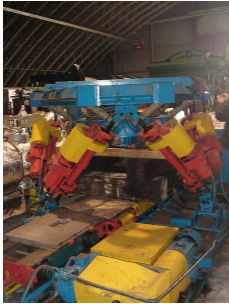
\includegraphics[scale=1]{Robot 1.PNG} \\

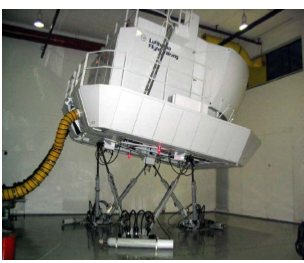
\includegraphics[scale=1]{Roboto 2.PNG}\\
\begin{flushleft}
Los robots anteriores representan las aplicaciones iniciales de los robot paralelos, pero no es hasta el año 1987 que los robot paralelos vuelven a tener un auge en la comunidad científica y de desarrollo de aplicaciones (Merlet, 2000). En el siguiente apartado se presentan diversos robots agrupados por campos de aplicación. 
\begin{center}
APLICACIONES DE PICK AND PLACE (RECOGER Y COLOCAR) 
\begin{flushleft}
La aplicación más conocida y desarrollada de estos robot es en  operaciones de pick and place. Es de destacar que el robot serial equivalente para este tipo de operaciones lo constituye el robot SCARA (Selective Compliant Assembly Robot Arms) que presenta 4 GdL. Un robot SCARA permite posicionar el elemento terminal, y por ende la pieza, en el espacio cartesiano,  además también puede realizar una rotación.\\
  El robot fue desarrollado partiendo de la idea de desarrollar un robot para manipular objetos de bajo peso a altas velocidades. La particularidad del robot Delta es que la plataforma móvil va unida a la base mediante 3 piernas donde cada pierna presenta un mecanismo de paralelogramo que permite balancear el centro de masa de cada una de ellas.
  \begin{center}
  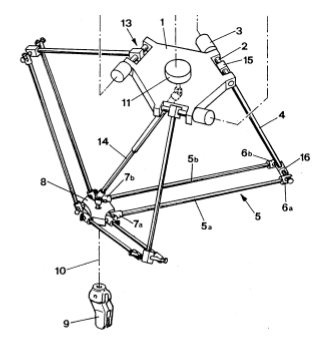
\includegraphics[scale=1]{Robot 3.PNG} 
  \begin{flushleft}
  Existen otros desarrollos de robot paralelos para aplicaciones del tipo SCARA pero estos no han alcanzado su aplicación comercial y se mantienen a nivel de desarrollo de laboratorios de investigación o universidades, entre ellos el lector interesado puede consultar [11], [14]-[16] por mencionar solo algunos. 
  \begin{center}
  APLICACIONES EN CENTRO DE MECANIZADO
  \begin{flushleft}
  Otra de las aplicaciones prácticas de los robots paralelos se encuentra en el área de desarrollo de centros de mecanizado. En este campo es común que los desarrolladores se refieran al robot paralelo como Mecanismo Cinemático Paralelo (MCP) en inglés Parallel Kinematic Mechanism (PKM). 
  \begin{center}
  APLICACIONES EN LA CIRUGÍA ROBÓTICA 
  \begin{flushleft}
  La cirugía mínimamente invasiva representa una de las áreas donde la introducción de robot 
produce un gran impacto, sobre todo mejorando las prestaciones de la cirugía laparoscópica, ya que aumenta la habilidad del cirujano a la hora de realizar una operación (mayor precisión, evita el movimiento errático del pulso de la mano).  Con la cirugía robótica se han logrado avances como realizar una operación mediante orificios de 10 mm en el cuerpo del paciente.\\
El mecanismo se caracteriza por tener juntas de revoluta, los autores presentan el diseño óptimo del robot mediante algoritmos genéticos. Sin embargo este robot no ha evolucionado más allá de su diseño preliminar.
\begin{center}
APLICACIONES EN ROBÓTICA PARA REHABILITACIÓN
\begin{flushleft}
La rehabilitación robótica se presenta como otro de los campos de  mayor interés en la actualidad, sirviendo de asistencia al trabajo arduo  de los fisioterapeutas, además de que logra una mejor coordinación para  los ejercicios de rehabilitación y mayor precisión en el diagnóstico de  lesiones y la medición de la evolución de los pacientes. La rehabilitación y diagnosis de las extremidades inferiores es muy frecuente debido a la  gran cantidad de accidentes a los que están expuestas estas extremidades,  de hecho, en el campo de los deportes suelen presentarse muy a menudo. 
\begin{center}
APLICACIONES EN EL LABORATORIO UPV Y MECABOT-ULA
\begin{flushleft}
El Laboratorio de Mecatrónica y Robótica de la Universidad de los Andes (MECABOT-ULA),  Venezuela, conjuntamente con grupos de investigación de la Universitàt Politècnica de Valencia han venido desarrollando metodologías para el diseño de sistemas biomecatrónicos para el diagnóstico y rehabilitación de extremidades del cuerpo humano. En particular, se han desarrollado y construido 
dos prototipos robóticos para rehabilitación y diagnosis de la extremidad inferior.  El primer robot fue enfocado para cubrir con tareas de rehabilitación del tobillo, el robot presenta una arquitectura donde la plataforma móvil va unida a la base mediante 3 piernas de configuración PRS. El desarrollo mecatrónico que incluye el modelo cinemático y dinámico del robot puede ser consultado en.
\begin{flushleft}
 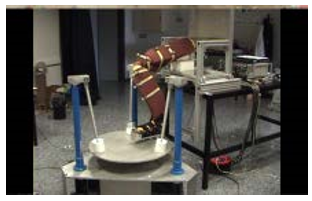
\includegraphics[scale=1]{Robot 4.PNG}
 \begin{flushleft}
  El diseño mecatrónico basado en un controlador PID se puede consultar en. El robot está en la fase preliminar, faltando la etapa de identificación de parámetros y el desarrollo de controladores basados en el modelo dinámico. Cada pierna es actuada en el par prismático por medio de un sistema de motor y tornillo de potencia.
  \end{flushleft} 
 \end{flushleft} 
\end{flushleft}
\end{center}
\end{flushleft}
\end{center}
  \end{flushleft}
  \end{center}
  \end{flushleft}
  \end{center}
  \end{flushleft}
  \end{center}
\end{flushleft}
\end{center}
\end{flushleft}

\end{flushleft}
\end{document}